2024年7月14日晚,于法喜寺旁发现了蚰蜒,其奇特的外观以及外号引起了我们的注意。

蚰蜒体短而微扁,棕黄色,体长1-6厘米,主要由头部及毒牙、触角、背板、腹板、15对步足和内脏团等部分组成。
头部两侧对称生长着由大量单眼组成的伪复眼。头部最前端生有两根触角。它的身体共有15节腹板,相邻两节之间上下重叠,以鱼鳞状排列。
背板也呈分节结构,同样以鱼鳞状排列。全身每节都长有一对细长的步足。

\begin{figure}[H]
    \centering
    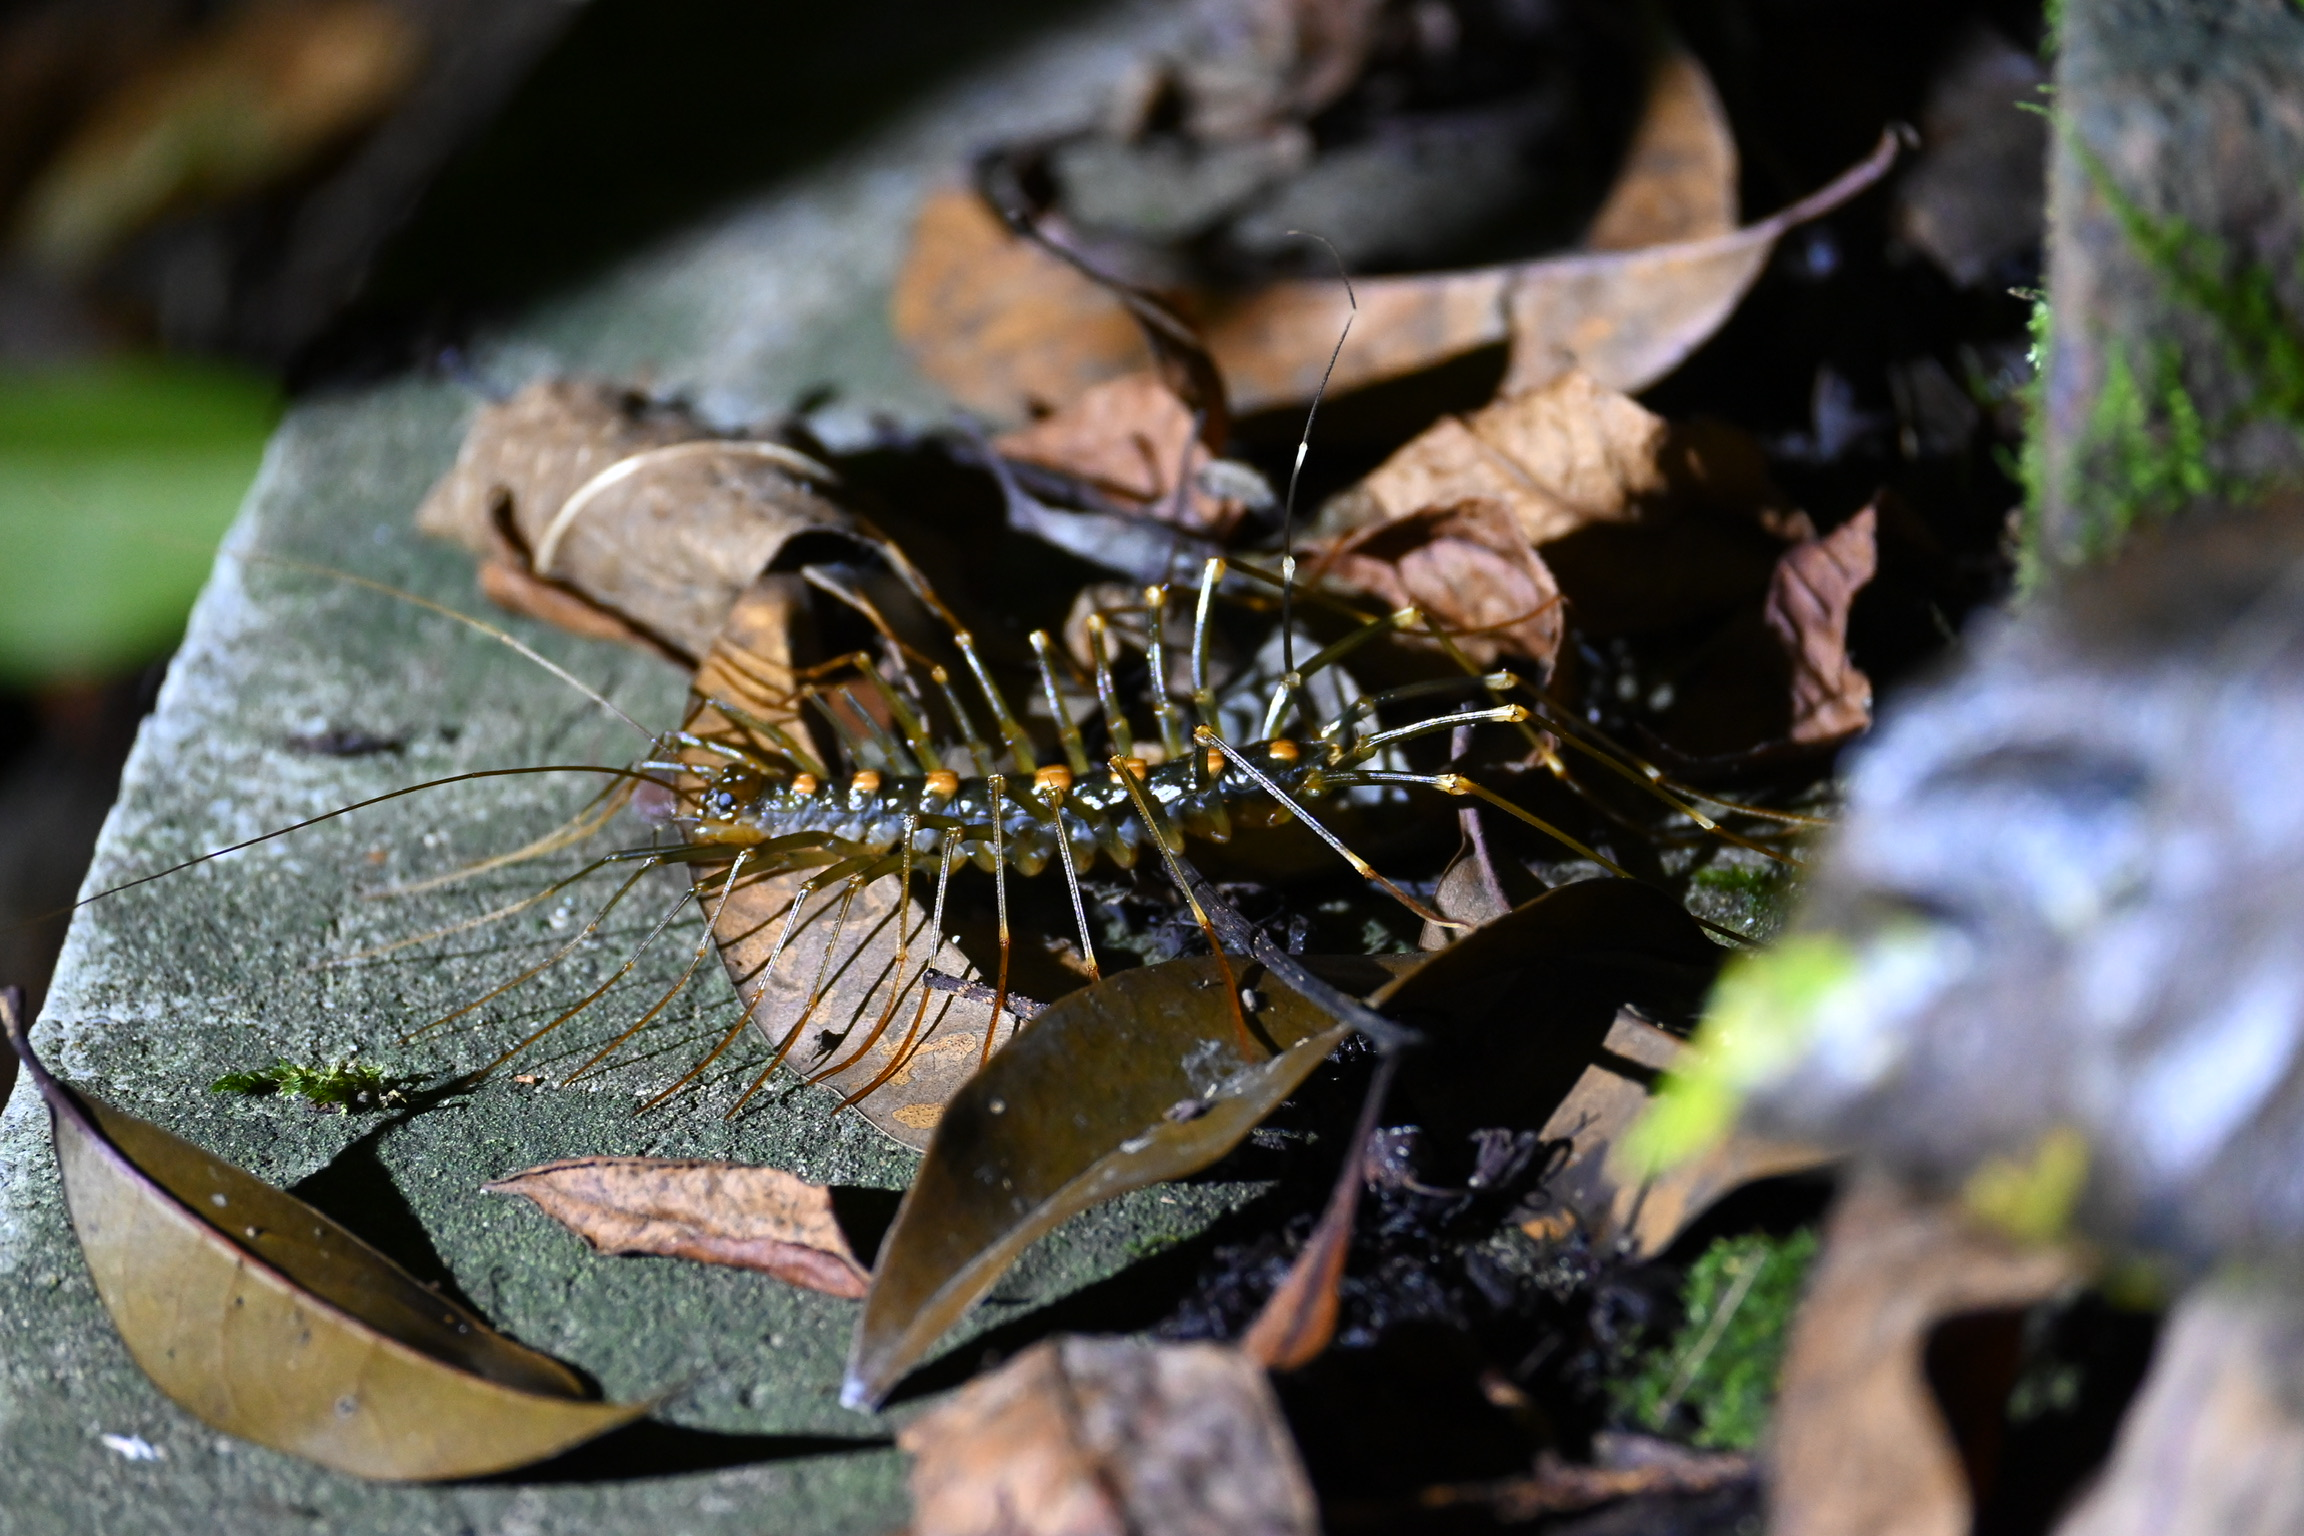
\includegraphics[width = .8\textwidth]{../assets/微信图片_20250226160858.jpg}
    \caption{拍摄到的蚰蜒图片}
\end{figure}